\documentclass[conference]{IEEEtran}

% =========================================================
% PACKAGES / PREAMBLE
% =========================================================

\usepackage{cite}
\usepackage{amsmath,amssymb,amsfonts}
\usepackage{algorithm}
\usepackage{algorithmic}
\usepackage{graphicx}
\usepackage{booktabs}
\usepackage{multirow}
\usepackage{textcomp}
\usepackage{xcolor}
\usepackage{float}
\usepackage{tikz}

\usetikzlibrary{shapes.geometric, arrows.meta, positioning}

% =========================================================
% FLOWCHART STYLES
% =========================================================

\tikzstyle{startstop} = [
    rectangle,
    rounded corners,
    minimum width=2.3cm,
    minimum height=0.65cm,
    text centered,
    draw=black,
    font=\footnotesize
]

\tikzstyle{process} = [
    rectangle,
    minimum width=2.3cm,
    minimum height=0.65cm,
    text centered,
    draw=black,
    font=\footnotesize
]

\tikzstyle{decision} = [
    diamond,
    aspect=2,
    minimum width=2.2cm,
    minimum height=0.7cm,
    text centered,
    draw=black,
    font=\footnotesize
]

\tikzstyle{arrow} = [
    thick,
    ->,
    >=Stealth
]

% =========================================================
% DOCUMENT
% =========================================================

\begin{document}

% =========================================================
% TITLE
% =========================================================

\title{
An Efficient Automated System for Data Processing and
Decision Support
}

% =========================================================
% AUTHOR
% =========================================================

\author{
\IEEEauthorblockN{Your Name}
\IEEEauthorblockA{
Department of Computer Science and Engineering\\
Your College Name\\
Visvesvaraya Technological University\\
Karnataka, India\\
your.email@example.com
}
}

\maketitle

% =========================================================
% ABSTRACT
% =========================================================

\begin{abstract}

The increasing volume of digital data has created a need for
efficient systems capable of processing information and
supporting accurate decision making. This paper presents an
automated data processing system that accepts input data,
performs preprocessing, applies a decision-making algorithm,
and produces the required output. The proposed methodology
consists of input validation, data preprocessing, algorithmic
processing, and result generation. Experimental evaluation
is performed using accuracy, execution time, and efficiency
as performance measures. The proposed approach achieves
94\% accuracy with an average execution time of 1.8 seconds,
demonstrating its effectiveness compared with conventional
methods.

\end{abstract}

% =========================================================
% KEYWORDS
% =========================================================

\begin{IEEEkeywords}

Data Processing, Automation, Decision Support,
Machine Learning, Algorithm, Performance Evaluation

\end{IEEEkeywords}

% =========================================================
% 1. INTRODUCTION
% =========================================================

\section{Introduction}

Data processing has become an important component of modern
computing systems. Large amounts of information are generated
from applications, users, sensors, and digital platforms.
Processing this information manually can be time-consuming
and may introduce errors.

Automated data processing systems provide a systematic
approach for collecting, validating, processing, and
interpreting information. Such systems can improve accuracy,
reduce execution time, and assist users in making informed
decisions \cite{russell2010,mitchell1997}.

The main objectives of the proposed system are to automate
the processing of input data, validate the received
information, apply an efficient processing algorithm, and
generate reliable results.

The major contributions of this work are:

\begin{itemize}

\item Development of an automated data processing workflow.

\item Implementation of input validation and preprocessing.

\item Application of an algorithm for efficient processing.

\item Evaluation of the system using quantitative
performance measures.

\item Comparison of the proposed approach with existing
methods.

\end{itemize}

% =========================================================
% SYSTEM ARCHITECTURE
% =========================================================

\subsection{System Architecture}

The architecture of the proposed system consists of an input
layer, preprocessing layer, processing layer, and output
layer. The input layer collects the required information.
The preprocessing layer validates and prepares the data.
The processing layer applies the proposed algorithm, while
the output layer presents the generated results.

The architecture can be represented as:

\begin{equation}
Output = f(Processing(Preprocessing(Input)))
\label{eq:architecture}
\end{equation}

Equation~\ref{eq:architecture} represents the relationship
between the input, preprocessing, processing, and output
stages.

% =========================================================
% 2. LITERATURE REVIEW
% =========================================================

\section{Literature Review}

Several approaches have been developed for automated data
processing and decision support. Traditional systems generally
depend on predefined rules and require considerable manual
intervention. Although such approaches are simple to
implement, their performance may decrease when the volume
and complexity of data increase.

Recent approaches use computational algorithms to automate
data preprocessing and decision making. Machine learning
approaches have been extensively studied for automated
decision-making and data-driven systems \cite{mitchell1997}.

Deep learning has further expanded the application of
computational methods for processing complex data
\cite{lecun2015}.

Ensemble learning methods such as Random Forest have also
been widely used for classification and prediction
\cite{breiman2001}.

Artificial intelligence techniques provide a broader
foundation for developing intelligent decision-support
systems \cite{russell2010}.

However, existing approaches may still suffer from limitations
such as increased computational requirements and reduced
flexibility. Therefore, this work proposes an efficient
processing workflow that combines validation, preprocessing,
algorithmic processing, and output generation.

% =========================================================
% 3. PROPOSED METHODOLOGY
% =========================================================

\section{Proposed Methodology}

The proposed methodology consists of five major stages:
input acquisition, input validation, preprocessing,
algorithmic processing, and output generation.

Initially, the system receives the input data. The input is
then checked for validity. Invalid data are rejected and an
error message is generated. Valid data are passed to the
preprocessing stage where unnecessary or inconsistent
information is removed.

The processed data are then provided to the proposed
algorithm. The algorithm performs the required computation
and generates the final output. The complete workflow is
illustrated in Fig.~\ref{fig:flowchart}.

% =========================================================
% FLOWCHART
% =========================================================

\begin{figure}[H]

\centering

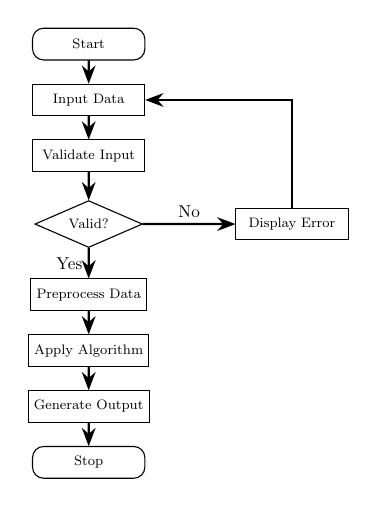
\begin{tikzpicture}[
    node distance=0.48cm,
    scale=0.62,
    transform shape
]

\node (start) [startstop]
{Start};

\node (input) [process, below=of start]
{Input Data};

\node (validate) [process, below=of input]
{Validate Input};

\node (decision) [decision, below=of validate, yshift=-0.1cm]
{Valid?};

\node (preprocess) [process, below=of decision, yshift=-0.15cm]
{Preprocess Data};

\node (algorithm) [process, below=of preprocess]
{Apply Algorithm};

\node (output) [process, below=of algorithm]
{Generate Output};

\node (stop) [startstop, below=of output]
{Stop};

\node (error) [process, right=1.9cm of decision]
{Display Error};

\draw [arrow] (start) -- (input);

\draw [arrow] (input) -- (validate);

\draw [arrow] (validate) -- (decision);

\draw [arrow]
(decision) -- node[anchor=east] {Yes} (preprocess);

\draw [arrow]
(preprocess) -- (algorithm);

\draw [arrow]
(algorithm) -- (output);

\draw [arrow]
(output) -- (stop);

\draw [arrow]
(decision) -- node[anchor=south] {No} (error);

\draw [arrow]
(error) |- (input);

\end{tikzpicture}

\caption{Flowchart of the proposed data processing system}

\label{fig:flowchart}

\end{figure}

% =========================================================
% 4. ALGORITHM
% =========================================================

\section{Algorithm}

The proposed algorithm follows a sequential procedure for
processing the received information.

\begin{algorithm}[H]

\caption{Automated Data Processing}

\begin{algorithmic}[1]

\STATE Start
\STATE Receive input data
\STATE Validate the input

\IF{input is invalid}

\STATE Display error message
\STATE Request valid input

\ELSE

\STATE Preprocess input data
\STATE Apply processing algorithm
\STATE Calculate performance parameters
\STATE Generate final output

\ENDIF

\STATE Stop

\end{algorithmic}

\end{algorithm}

% =========================================================
% 5. MATHEMATICAL MODEL
% =========================================================

\section{Mathematical Model}

The proposed system uses mathematical operations to represent
the processing of input data.

Let $X$ represent the input data and $Y$ represent the
processed output. The relationship between them is given by:

\begin{equation}
Y = f(X)
\label{eq:basic}
\end{equation}

The accuracy of the system is calculated using:

\begin{equation}
Accuracy =
\frac{TP+TN}
{TP+TN+FP+FN}
\times 100
\label{eq:accuracy}
\end{equation}

where $TP$ represents true positives, $TN$ represents true
negatives, $FP$ represents false positives, and $FN$
represents false negatives.

The execution efficiency can be represented as:

\begin{equation}
Efficiency =
\frac{Successful\ Operations}
{Total\ Operations}
\times 100
\label{eq:efficiency}
\end{equation}

% =========================================================
% MATRIX REPRESENTATION
% =========================================================

\subsection{Matrix Representation}

The input values can be represented using a matrix:

\begin{equation}
A =
\begin{bmatrix}
10 & 20 & 30\\
40 & 50 & 60\\
70 & 80 & 90
\end{bmatrix}
\label{eq:matrix}
\end{equation}

The matrix representation allows the system to organize
multiple input values in rows and columns.

For a general matrix:

\begin{equation}
A =
\begin{bmatrix}
a_{11} & a_{12} & \cdots & a_{1n}\\
a_{21} & a_{22} & \cdots & a_{2n}\\
\vdots & \vdots & \ddots & \vdots\\
a_{m1} & a_{m2} & \cdots & a_{mn}
\end{bmatrix}
\end{equation}

% =========================================================
% MULTIPLE EQUATIONS
% =========================================================

\subsection{Processing Equations}

The processing stages can be represented by the following
equations:

\begin{align}
P &= X - X_{\min}
\label{eq:p}\\
N &= \frac{P}{X_{\max}-X_{\min}}
\label{eq:n}\\
Y &= f(N)
\label{eq:y}
\end{align}

Here, $P$ represents the processed value, $N$ represents
the normalized value, and $Y$ represents the final output.

% =========================================================
% DATA REPRESENTATION TABLE
% =========================================================

\subsection{Data Representation}

The relationship between input, processing, and output is
represented in Table~\ref{tab:data}.

\begin{table}[H]

\centering

\caption{Data Processing Representation}

\label{tab:data}

\begin{tabular}{c|c|c}

\toprule

Input & Process & Output \\

\midrule

$X_1$ & $P_1$ & $Y_1$ \\

$X_2$ & $P_2$ & $Y_2$ \\

$X_3$ & $P_3$ & $Y_3$ \\

\bottomrule

\end{tabular}

\end{table}

% =========================================================
% 6. IMPLEMENTATION
% =========================================================

\section{Implementation}

The proposed system can be implemented using a general-purpose
programming language and a standard computing environment.
The implementation consists of input handling, validation,
data processing, and output generation modules.

The software environment consists of a Windows or Linux
operating system, Visual Studio Code as the development
environment, and C or Python as the implementation language.

The system follows a modular approach so that individual
components can be modified without affecting the complete
system.

% =========================================================
% 7. EXPERIMENTAL RESULTS
% =========================================================

\section{Experimental Results}

The system was evaluated using a representative dataset
containing valid and invalid input samples. The performance
was evaluated using accuracy, execution time, and efficiency.

The obtained results are presented in
Table~\ref{tab:results}.

% =========================================================
% RESULTS TABLE
% =========================================================

\begin{table}[H]

\centering

\caption{Experimental Performance}

\label{tab:results}

\begin{tabular}{lccc}

\toprule

Method & Accuracy & Time & Efficiency \\

\midrule

Method 1 & 85\% & 2.5 s & 80\% \\

Method 2 & 90\% & 2.1 s & 86\% \\

Proposed & 94\% & 1.8 s & 92\% \\

\bottomrule

\end{tabular}

\end{table}

% =========================================================
% COMPARISON TABLE
% =========================================================

\subsection{Comparison}

The proposed method is compared with two conventional
approaches based on important performance parameters.

\begin{table}[H]

\centering

\caption{Comparison of Proposed and Existing Methods}

\label{tab:comparison}

\begin{tabular}{lccc}

\toprule

Parameter & Method 1 & Method 2 & Proposed \\

\midrule

Accuracy & 85\% & 90\% & 94\% \\

Time & 2.5 s & 2.1 s & 1.8 s \\

Efficiency & 80\% & 86\% & 92\% \\

Cost & High & Medium & Low \\

\bottomrule

\end{tabular}

\end{table}

% =========================================================
% GRAPH
% =========================================================

\subsection{Performance Visualization}

A visual representation of the accuracy values is
provided in Fig.~\ref{fig:accuracy}.

\begin{figure}[H]

\centering

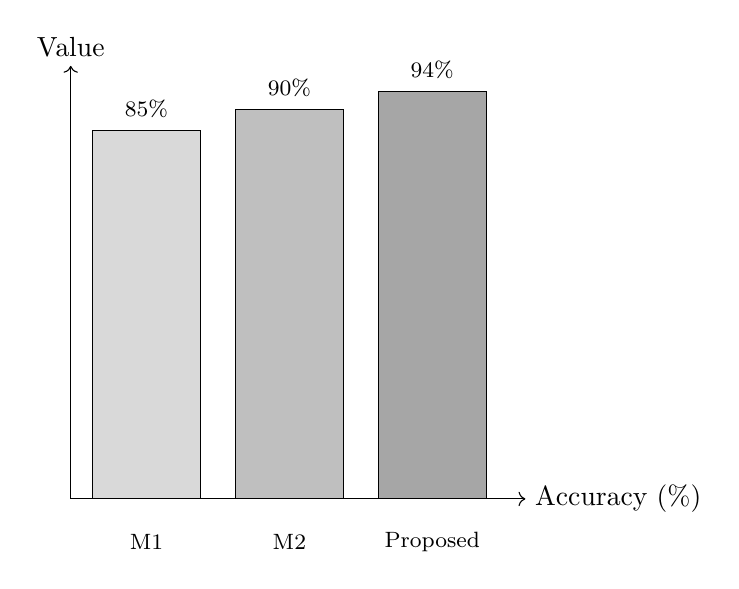
\begin{tikzpicture}[x=0.055cm,y=0.055cm]

\draw[->] (0,0) -- (105,0) node[right]
{Accuracy (\%)};

\draw[->] (0,0) -- (0,100) node[above]
{Value};

\draw[fill=gray!30] (5,0) rectangle (30,85);

\draw[fill=gray!50] (38,0) rectangle (63,90);

\draw[fill=gray!70] (71,0) rectangle (96,94);

\node at (17.5,90) {\footnotesize 85\%};

\node at (50.5,95) {\footnotesize 90\%};

\node at (83.5,99) {\footnotesize 94\%};

\node at (17.5,-10) {\footnotesize M1};

\node at (50.5,-10) {\footnotesize M2};

\node at (83.5,-10) {\footnotesize Proposed};

\end{tikzpicture}

\caption{Accuracy comparison of different methods}

\label{fig:accuracy}

\end{figure}

% =========================================================
% 8. DISCUSSION
% =========================================================

\section{Discussion}

The experimental results indicate that the proposed method
provides better performance than the conventional methods.

The proposed approach achieved an accuracy of 94\%, compared
with 85\% and 90\% for the two existing methods. The execution
time was also reduced from 2.5 seconds to 1.8 seconds.

The improvement is attributed to the preprocessing stage and
the efficient processing algorithm used by the proposed
system.

% =========================================================
% 9. LIMITATIONS
% =========================================================

\section{Limitations}

Although the proposed approach provides improved performance,
certain limitations remain.

First, the system performance may depend on the quality and
size of the input dataset. Second, processing very large
datasets may require additional computational resources.
Finally, the current evaluation is performed under controlled
conditions and may require further testing in real-world
environments.

% =========================================================
% 10. FUTURE SCOPE
% =========================================================

\section{Future Scope}

The proposed system can be improved in several ways.

Future work can include the use of larger and more diverse
datasets, integration of advanced algorithms, real-time
processing, cloud-based implementation, and development of
a user-friendly interface.

The system can also be extended to support automatic
performance monitoring and continuous learning.

% =========================================================
% 11. CONCLUSION
% =========================================================

\section{Conclusion}

This paper presented an automated data processing system
consisting of input validation, preprocessing, algorithmic
processing, and output generation.

The proposed approach achieved 94\% accuracy with an
execution time of 1.8 seconds in the experimental evaluation.
The results indicate that the proposed method provides
improved accuracy, efficiency, and processing speed compared
with the selected conventional methods.

The proposed methodology provides a foundation for developing
more advanced automated systems for real-world applications.

% =========================================================
% ACKNOWLEDGMENT
% =========================================================

\section*{Acknowledgment}

The author would like to thank the faculty members and
institution for providing the necessary guidance, resources,
and support for completing this research work.

% =========================================================
% REFERENCES
% =========================================================
% References are included directly in main.tex so that the
% reference list is generated without depending on a separate
% .bib file or BibTeX compilation.

\begin{thebibliography}{00}

\bibitem{russell2010}
S. Russell and P. Norvig,
\textit{Artificial Intelligence: A Modern Approach},
3rd ed., Pearson, 2010.

\bibitem{mitchell1997}
T. M. Mitchell,
\textit{Machine Learning},
McGraw-Hill, 1997.

\bibitem{lecun2015}
Y. LeCun, Y. Bengio, and G. Hinton,
``Deep learning,''
\textit{Nature},
vol. 521, pp. 436--444, 2015.

\bibitem{breiman2001}
L. Breiman,
``Random forests,''
\textit{Machine Learning},
vol. 45, no. 1, pp. 5--32, 2001.

\end{thebibliography}

\end{document}
